\documentclass[conference]{IEEEtran}
\IEEEoverridecommandlockouts
% Paquetes para español
\usepackage[spanish]{babel}
\usepackage[utf8]{inputenc}
\usepackage{cite}
\usepackage{amsmath,amssymb,amsfonts}
\usepackage{algorithmic}
\usepackage{graphicx}
\usepackage{textcomp}
\usepackage{booktabs}
\usepackage{xcolor}
\usepackage{array}
\usepackage{iftex}
% Con XeLaTeX/LuaLaTeX (p. ej. Tectonic) se carga una fuente tipo Times con negritas y cursivas;
% con pdfLaTeX se conserva la fuente estándar de IEEEtran
\ifPDFTeX\else
  \usepackage{fontspec}
  \setmainfont{texgyretermes}[Extension=.otf, UprightFont=*-regular, BoldFont=*-bold, ItalicFont=*-italic, BoldItalicFont=*-bolditalic]
\fi
% Si falta una imagen, muestra un recuadro en lugar de detener la compilación
\let\oldincludegraphics\includegraphics
\renewcommand{\includegraphics}[2][]{\IfFileExists{#2}{\oldincludegraphics[#1]{#2}}{\fbox{\parbox{0.8\columnwidth}{\centering Imagen faltante:\\ \texttt{\detokenize{#2}}}}}}
\def\BibTeX{{\rm B\kern-.05em{\sc i\kern-.025em b}\kern-.08em
    T\kern-.1667em\lower.7ex\hbox{E}\kern-.125emX}}
\begin{document}

\title{Entrenamiento de una red neuronal multicapa mediante filtro extendido de Kalman}

\author{\IEEEauthorblockN{1\textsuperscript{st} Oscar Alberto Gallo García}
\IEEEauthorblockA{\textit{M. C. en Robótica e Inteligencia Artificial} \\
\textit{Centro Universitario de Ciencias Exactas e Ingenierías}\\
Guadalajara, México \\
oscar.gallo5770@alumnos.udg.mx}
}

\maketitle

\begin{abstract}
    Se retomó el perceptrón multicapa 2--6--4 de la práctica anterior, que
    clasifica a adultos de la ENSANUT 2022 en las cuatro categorías de índice
    de masa corporal a partir de su altura y su peso, y se sustituyó el
    entrenamiento por retropropagación con descenso de gradiente por un
    entrenamiento basado en el filtro extendido de Kalman (EKF),
    implementado desde cero. Los $46$ pesos y sesgos se agruparon en un único
    vector de parámetros, se construyó la matriz Jacobiana de las salidas
    respecto a dicho vector mediante la regla de la cadena y se aplicaron las
    ecuaciones de ganancia, corrección de pesos y actualización de la
    covarianza. Con $p_0=100$, $q=0.001$, $r=1$ y $\eta=1$, el EKF redujo la
    energía promedio del error de $0.0293$ a $0.0052$ en $20$ épocas y alcanzó
    $99.44\%$ de exactitud de prueba, frente a $0.0266$ y $97.12\%$ obtenidos
    por retropropagación en $200$ épocas con los mismos pesos iniciales. El
    EKF reconoció además los $15$ patrones de prueba de la clase bajo peso,
    que retropropagación no detectó. Cada época del EKF fue $5.7$ veces más
    costosa, pero el tiempo total resultó menor, $30.2$ s contra $53.3$ s,
    por requerir diez veces menos épocas.
\end{abstract}

\begin{IEEEkeywords}
Filtro extendido de Kalman, perceptrón multicapa, estimación de parámetros, matriz Jacobiana, retropropagación, clasificación multiclase, IMC
\end{IEEEkeywords}

\section{Introducción}
En la práctica anterior se entrenó un perceptrón multicapa mediante
retropropagación: se define una función de costo, se calcula su gradiente
respecto a cada peso y los pesos se modifican en la dirección que reduce
dicho costo. El procedimiento es de primer orden y su velocidad depende de
una única razón de aprendizaje, común a todos los parámetros.

Los filtros de Kalman se desarrollaron originalmente para la estimación de
estados de sistemas dinámicos. En el entrenamiento de redes neuronales se
utiliza una interpretación equivalente, en la cual los pesos de la red son
las variables que se desea estimar y la salida deseada de cada patrón
desempeña el papel de la medición \cite{b1,b2,b3,b4}. Dado que el mapeo
entrada--salida de una red multicapa es no lineal, se emplea el filtro
extendido de Kalman (EKF), que linealiza dicho mapeo alrededor de los pesos
actuales mediante el Jacobiano de las salidas respecto a los pesos
\cite{b5,b7}. A diferencia del descenso de gradiente, el EKF mantiene una
matriz de covarianza que representa la incertidumbre de cada parámetro y
las correlaciones entre ellos, con la cual calcula una corrección adaptativa
para cada patrón.

En esta práctica se conservan la arquitectura, los datos, el
preprocesamiento, la partición y los pesos iniciales de la Práctica~3, de
modo que la única variable que cambia es el algoritmo de entrenamiento. El
objetivo es implementar las ecuaciones del EKF desde cero y comparar
experimentalmente ambos esquemas en convergencia, generalización, tiempo de
cómputo, memoria y sensibilidad a los parámetros de diseño.

\section{Desarrollo}

\subsection{Red y datos reutilizados de la Práctica 3}
Se utilizó la misma base de antropometría de la ENSANUT 2022 \cite{b6} y la
misma limpieza: adultos de $20$ a $110$ años, sin embarazo ni lactancia,
con peso entre $2$ y $250$ kg y estatura entre $40$ y $230$ cm. Tras la
limpieza quedaron $N=6\,246$ registros. La entrada de la red es
$\mathbf{X}(k)=[\text{altura}(k),\ \text{peso}(k)]^\top$ y el IMC se empleó
únicamente para construir la etiqueta de cada patrón:
\begin{align}
    \label{eq:clases}
    \begin{aligned}
    C_1&:\ \text{Bajo peso}, &&\text{IMC}<18.5,\\
    C_2&:\ \text{Peso normal}, &&18.5\leq\text{IMC}<25,\\
    C_3&:\ \text{Sobrepeso}, &&25\leq\text{IMC}<30,\\
    C_4&:\ \text{Obesidad}, &&\text{IMC}\geq30.
    \end{aligned}
\end{align}
La salida deseada $\mathbf{d}(k)\in\mathbb{R}^4$ se representó con
codificación \textit{one-hot} y la clase predicha corresponde a la neurona
de salida con mayor activación. El Cuadro~\ref{tab:clases} muestra la
distribución de patrones, en la que destaca el desbalance de la clase
$C_1$, con solo el $1.36\%$ de los datos.

\begin{table}[htbp]
\caption{Distribución de patrones por clase}
\label{tab:clases}
\begin{center}
\begin{tabular}{lrrrr}
\toprule
\textbf{Clase} & \textbf{Total} & \textbf{\%} & \textbf{Entren.} & \textbf{Prueba} \\
\midrule
$C_1$ Bajo peso   & $85$     & $1.36$  & $70$     & $15$  \\
$C_2$ Peso normal & $1\,286$ & $20.59$ & $1\,031$ & $255$ \\
$C_3$ Sobrepeso   & $2\,288$ & $36.63$ & $1\,834$ & $454$ \\
$C_4$ Obesidad    & $2\,587$ & $41.42$ & $2\,062$ & $525$ \\
\midrule
Total             & $6\,246$ & $100$   & $4\,997$ & $1\,249$ \\
\bottomrule
\end{tabular}
\end{center}
\end{table}

Se conservó la partición de $80\%$ para entrenamiento y $20\%$ para prueba
con semilla fija, y las entradas se estandarizaron con la media y la
desviación estándar del conjunto de entrenamiento, $\mu_1=1.5946$ m,
$\sigma_1=0.1076$ m, $\mu_2=75.181$ kg y $\sigma_2=19.570$ kg. Los mismos
parámetros se aplicaron al conjunto de prueba.

La arquitectura es 2--6--4: $p=2$ entradas, una capa oculta con $N_h=6$
neuronas y $m=4$ salidas. Ambas capas utilizan la sigmoide logística,
\begin{align}
    \label{eq:sigmoide}
    \varphi(v)=\frac{1}{1+e^{-v}},\qquad \varphi'(v)=\varphi(v)\left[1-\varphi(v)\right].
\end{align}
Con $y_i^{(0)}(k)=x_i(k)$, la propagación hacia adelante de la capa
$\ell\in\{1,2\}$ es
\begin{align}
    \label{eq:v}
    v_j^{(\ell)}(k)&=\sum_{i} w_{ji}^{(\ell)}(k)\,y_i^{(\ell-1)}(k)+b_j^{(\ell)}(k),\\
    \label{eq:y}
    y_j^{(\ell)}(k)&=\varphi\!\left(v_j^{(\ell)}(k)\right),
\end{align}
y la salida de la red es $\widehat{\mathbf{y}}(k)=\mathbf{y}^{(2)}(k)$. Los
pesos y sesgos se inicializaron con distribución uniforme en $(-1,1)$ y
semilla $42$, de manera que ambos algoritmos parten exactamente de los
mismos valores.

\subsection{Vector de parámetros}
El EKF actualiza todos los parámetros de la red mediante un único vector.
Se definió
\begin{align}
    \label{eq:w}
    \mathbf{w}(k)=
    \begin{bmatrix}
    \operatorname{vec}\!\left(\mathbf{W}^{(1)}\right)\\[2pt]
    \mathbf{b}^{(1)}\\[2pt]
    \operatorname{vec}\!\left(\mathbf{W}^{(2)}\right)\\[2pt]
    \mathbf{b}^{(2)}
    \end{bmatrix}\in\mathbb{R}^{L},
\end{align}
donde $\operatorname{vec}(\cdot)$ recorre cada matriz fila por fila. El
número total de parámetros es
\begin{align}
    \label{eq:L}
    L=(p+1)N_h+(N_h+1)m=3\cdot6+7\cdot4=46.
\end{align}
El Cuadro~\ref{tab:orden} documenta el orden elegido. Este orden es único y
se utiliza en tres lugares: al empaquetar los pesos en $\mathbf{w}$, al
construir las filas del Jacobiano y al regresar el vector actualizado a las
matrices de la red. En el código, estas tres operaciones se realizan en
los métodos \texttt{weight2vector}, \texttt{jacobian} y
\texttt{vector2weight}, respectivamente.
Se verificó que empaquetar y desempaquetar de forma consecutiva deja los
parámetros sin cambio.

\begin{table}[htbp]
\caption{Orden de los parámetros en el vector $\mathbf{w}$}
\label{tab:orden}
\begin{center}
\begin{tabular}{clcc}
\toprule
\textbf{Posiciones} & \textbf{Contenido} & \textbf{Forma} & \textbf{Cantidad} \\
\midrule
$1$--$12$  & $\mathbf{W}^{(1)}$, pesos de la capa oculta   & $6\times2$ & $12$ \\
$13$--$18$ & $\mathbf{b}^{(1)}$, sesgos de la capa oculta  & $6\times1$ & $6$ \\
$19$--$42$ & $\mathbf{W}^{(2)}$, pesos de la capa de salida  & $4\times6$ & $24$ \\
$43$--$46$ & $\mathbf{b}^{(2)}$, sesgos de la capa de salida & $4\times1$ & $4$ \\
\bottomrule
\end{tabular}
\end{center}
\end{table}

\subsection{Entrenamiento como estimación de parámetros}
Los pesos se consideran parámetros desconocidos cuya evolución se modela
como
\begin{align}
    \label{eq:proceso}
    \mathbf{w}(k+1)=\mathbf{w}(k)+\mathbf{q}(k),
\end{align}
donde $\mathbf{q}(k)$ representa la incertidumbre permitida en los
parámetros y se relaciona con la matriz $\mathbf{Q}$. Para cada patrón, la
red completa actúa como la función de medición,
\begin{align}
    \label{eq:medicion}
    \widehat{\mathbf{y}}(k)=\mathbf{h}\!\left(\mathbf{w}(k),\mathbf{X}(k)\right),
\end{align}
y el error que dirige la corrección es la diferencia entre la salida
deseada conocida y la salida calculada,
\begin{align}
    \label{eq:error}
    \mathbf{e}(k)=\mathbf{d}(k)-\widehat{\mathbf{y}}(k)\in\mathbb{R}^{4}.
\end{align}
La definición del error es la misma que en retropropagación; lo que cambia
es la forma en que se utiliza para actualizar los pesos.

\subsection{Ecuaciones del EKF}
Con la orientación matricial $\mathbf{H}(k)\in\mathbb{R}^{L\times m}$, el
algoritmo es \cite{b1,b3}
\begin{align}
    \label{eq:K}
    \mathbf{K}(k)&=\mathbf{P}(k)\mathbf{H}(k)\left[\mathbf{R}+\mathbf{H}^\top(k)\mathbf{P}(k)\mathbf{H}(k)\right]^{-1},\\
    \label{eq:updw}
    \mathbf{w}(k+1)&=\mathbf{w}(k)+\eta\,\mathbf{K}(k)\,\mathbf{e}(k),\\
    \label{eq:updP}
    \mathbf{P}(k+1)&=\mathbf{P}(k)-\mathbf{K}(k)\mathbf{H}^\top(k)\mathbf{P}(k)+\mathbf{Q}.
\end{align}
Para la red utilizada las dimensiones son
$\mathbf{w}\in\mathbb{R}^{46\times1}$, $\mathbf{e}\in\mathbb{R}^{4\times1}$,
$\mathbf{H},\mathbf{K}\in\mathbb{R}^{46\times4}$,
$\mathbf{P},\mathbf{Q}\in\mathbb{R}^{46\times46}$ y
$\mathbf{R}\in\mathbb{R}^{4\times4}$. La matriz que se invierte en
\eqref{eq:K} es de $4\times4$, independientemente del número de pesos.

El significado de cada matriz es el siguiente. $\mathbf{P}(k)$ es la
covarianza del error de estimación de los pesos y representa la
incertidumbre asociada a los parámetros actuales. $\mathbf{Q}$ es la
covarianza del ruido de proceso; evita que $\mathbf{P}$ se anule y que el
estimador pierda su capacidad de adaptación. $\mathbf{R}$ es la covarianza
asociada al error de salida y regula cuánto peso se da a la innovación
instantánea $\mathbf{e}(k)$. Las tres se inicializaron de forma diagonal,
\begin{align}
    \label{eq:init}
    \mathbf{P}(0)=p_0\mathbf{I}_{L},\qquad \mathbf{Q}=q\,\mathbf{I}_{L},\qquad \mathbf{R}=r\,\mathbf{I}_{m}.
\end{align}

\subsection{Construcción de la matriz Jacobiana}
La matriz $\mathbf{H}(k)$ contiene la derivada de cada salida respecto a
cada parámetro; su columna $s$ es el gradiente de la salida
$\widehat{y}_s$ respecto a todo el vector de pesos,
\begin{align}
    \label{eq:H}
    \mathbf{H}(k)=
    \begin{bmatrix}
    \dfrac{\partial\widehat{y}_1}{\partial\mathbf{w}} & \dfrac{\partial\widehat{y}_2}{\partial\mathbf{w}} & \cdots & \dfrac{\partial\widehat{y}_m}{\partial\mathbf{w}}
    \end{bmatrix}\in\mathbb{R}^{L\times m}.
\end{align}

\textit{Pesos de la capa de salida.} Para la salida
$\widehat{y}_s=\varphi\!\left(v_s^{(2)}\right)$ y un peso $w_{rj}^{(2)}$, la
regla de la cadena da
\begin{align}
    \label{eq:cadena2}
    \frac{\partial\widehat{y}_s}{\partial w_{rj}^{(2)}}
    =\frac{\partial\widehat{y}_s}{\partial v_s^{(2)}}\,
     \frac{\partial v_s^{(2)}}{\partial w_{rj}^{(2)}}.
\end{align}
Un peso que llega a la neurona de salida $r$ solo modifica la salida de esa
neurona, de modo que la derivada es distinta de cero únicamente cuando
$r=s$:
\begin{align}
    \label{eq:dsalida}
    \frac{\partial\widehat{y}_s}{\partial w_{rj}^{(2)}}
    =\delta_{sr}\,\varphi'\!\left(v_s^{(2)}\right)y_j^{(1)},\qquad
    \frac{\partial\widehat{y}_s}{\partial b_{r}^{(2)}}
    =\delta_{sr}\,\varphi'\!\left(v_s^{(2)}\right),
\end{align}
donde $\delta_{sr}$ es la delta de Kronecker.

\textit{Pesos de la capa oculta.} Un peso $w_{ji}^{(1)}$ afecta de manera
indirecta a todas las salidas conectadas con la neurona oculta $j$:
\begin{align}
    \label{eq:cadena1}
    \frac{\partial\widehat{y}_s}{\partial w_{ji}^{(1)}}
    =\frac{\partial\widehat{y}_s}{\partial v_s^{(2)}}\,
     \frac{\partial v_s^{(2)}}{\partial y_j^{(1)}}\,
     \frac{\partial y_j^{(1)}}{\partial v_j^{(1)}}\,
     \frac{\partial v_j^{(1)}}{\partial w_{ji}^{(1)}}.
\end{align}
Sustituyendo cada término,
\begin{align}
    \label{eq:doculta}
    \frac{\partial\widehat{y}_s}{\partial w_{ji}^{(1)}}
    &=\varphi'\!\left(v_s^{(2)}\right)w_{sj}^{(2)}\,\varphi'\!\left(v_j^{(1)}\right)y_i^{(0)},\\
    \label{eq:dbias1}
    \frac{\partial\widehat{y}_s}{\partial b_{j}^{(1)}}
    &=\varphi'\!\left(v_s^{(2)}\right)w_{sj}^{(2)}\,\varphi'\!\left(v_j^{(1)}\right).
\end{align}

\textit{Forma programada.} Para cada salida $s$ se define la sensibilidad
$\Delta_j^{(\ell,s)}=\partial\widehat{y}_s/\partial v_j^{(\ell)}$, que se
calcula de forma recursiva desde la capa de salida:
\begin{align}
    \label{eq:sens2}
    \Delta_r^{(2,s)}&=\delta_{rs}\,\varphi'\!\left(v_r^{(2)}\right),\\
    \label{eq:sens1}
    \Delta_j^{(1,s)}&=\varphi'\!\left(v_j^{(1)}\right)\sum_{r=1}^{m}w_{rj}^{(2)}\,\Delta_r^{(2,s)},
\end{align}
con lo cual
$\partial\widehat{y}_s/\partial w_{ji}^{(\ell)}=\Delta_j^{(\ell,s)}\,y_i^{(\ell-1)}$
y $\partial\widehat{y}_s/\partial b_{j}^{(\ell)}=\Delta_j^{(\ell,s)}$. Estas
expresiones reproducen \eqref{eq:dsalida}--\eqref{eq:dbias1} y contienen los
mismos productos de derivadas que retropropagación. La diferencia es que en
retropropagación la recursión se inicia con el error
$e_j\,\varphi'(v_j^{(2)})$ y se ejecuta una sola vez para obtener el
gradiente del costo, mientras que aquí se inicia con un vector unitario por
cada salida y se ejecuta $m$ veces para obtener la sensibilidad de cada
salida por separado. Cada columna de $\mathbf{H}$ se ordena igual que el
Cuadro~\ref{tab:orden}. La implementación se validó comparando
$\mathbf{H}$ con un Jacobiano obtenido por diferencias finitas centradas,
con una diferencia máxima del orden de $10^{-10}$.

\subsection{Parámetros de diseño}
El Cuadro~\ref{tab:diseno} resume la configuración de ambos entrenamientos.
Los valores del EKF se eligieron con el siguiente criterio: $p_0$ grande
porque los pesos iniciales son aleatorios y su incertidumbre es alta; $q$
pequeño para conservar capacidad de adaptación sin inducir variaciones
innecesarias; $r=1$ como referencia para salidas en $[0,1]$; y $\eta=1$,
es decir, la corrección de Kalman sin atenuar. El efecto de modificar cada
uno se evalúa en la Sección~\ref{sec:sens}.

\begin{table}[htbp]
\caption{Parámetros de diseño de ambos entrenamientos}
\label{tab:diseno}
\begin{center}
\setlength{\tabcolsep}{4pt}
\begin{tabular}{lll}
\toprule
\textbf{Parámetro} & \textbf{Retropropagación} & \textbf{EKF} \\
\midrule
Arquitectura       & 2--6--4, $L=46$ & 2--6--4, $L=46$ \\
Activaciones       & Sigmoide logística & Sigmoide logística \\
Inicialización     & $\mathcal{U}(-1,1)$, semilla $42$ & $\mathcal{U}(-1,1)$, semilla $42$ \\
Orden de patrones  & Fijo & Fijo \\
Razón de aprendizaje & $\eta=0.01$ & $\eta=1$ \\
$\mathbf{P}(0)$    & --- & $p_0=100$ \\
$\mathbf{Q}$       & --- & $q=0.001$ \\
$\mathbf{R}$       & --- & $r=1$ \\
Épocas             & $200$ & $20$ \\
Criterio de paro   & Épocas fijas & Épocas fijas \\
\bottomrule
\end{tabular}
\end{center}
\end{table}

\subsection{Algoritmo}
El procedimiento se implementó en Python con NumPy, sin bibliotecas de
redes neuronales, de filtros de Kalman ni de diferenciación automática. La
covarianza $\mathbf{P}$ se inicializa una sola vez y se propaga entre
patrones y épocas.
\begin{algorithmic}[1]
\STATE Inicializar $\mathbf{W}^{(\ell)},\mathbf{b}^{(\ell)}\sim\mathcal{U}(-1,1)$
\STATE $\mathbf{P}\leftarrow p_0\mathbf{I}_{L}$,\ $\mathbf{Q}\leftarrow q\,\mathbf{I}_{L}$,\ $\mathbf{R}\leftarrow r\,\mathbf{I}_{m}$
\FOR{$n=1$ \TO $20$}
    \STATE $S\leftarrow0$
    \FOR{cada patrón $k$}
        \STATE $\mathbf{y}^{(0)}\leftarrow\mathbf{z}(k)$
        \FOR{$\ell=1$ \TO $2$}
            \STATE $\mathbf{y}^{(\ell)}\leftarrow\varphi(\mathbf{W}^{(\ell)}\mathbf{y}^{(\ell-1)}+\mathbf{b}^{(\ell)})$
        \ENDFOR
        \STATE $\mathbf{e}\leftarrow\mathbf{d}(k)-\mathbf{y}^{(2)}$
        \FOR{$s=1$ \TO $m$}
            \STATE Calcular $\boldsymbol{\Delta}^{(2,s)}$ y $\boldsymbol{\Delta}^{(1,s)}$ con \eqref{eq:sens2} y \eqref{eq:sens1}
            \STATE Columna $s$ de $\mathbf{H}$ $\leftarrow$ derivadas en el orden del Cuadro~\ref{tab:orden}
        \ENDFOR
        \STATE $\mathbf{K}\leftarrow\mathbf{P}\mathbf{H}\left[\mathbf{R}+\mathbf{H}^\top\mathbf{P}\mathbf{H}\right]^{-1}$
        \STATE $\mathbf{w}\leftarrow$ empaquetar pesos y sesgos
        \STATE $\mathbf{w}\leftarrow\mathbf{w}+\eta\,\mathbf{K}\,\mathbf{e}$
        \STATE Desempaquetar $\mathbf{w}$ en $\mathbf{W}^{(\ell)},\mathbf{b}^{(\ell)}$
        \STATE $\mathbf{P}\leftarrow\mathbf{P}-\mathbf{K}\mathbf{H}^\top\mathbf{P}+\mathbf{Q}$
        \STATE $\mathbf{P}\leftarrow(\mathbf{P}+\mathbf{P}^\top)/2$
        \STATE $S\leftarrow S+\tfrac{1}{2}\|\mathbf{e}\|^2$
    \ENDFOR
    \STATE $E_{\text{av}}(n)\leftarrow S/N$
    \STATE Registrar $\operatorname{tr}(\mathbf{P})$ y $\|\mathbf{K}\|$
\ENDFOR
\STATE Clasificar el conjunto de prueba con la salida de mayor activación
\end{algorithmic}
La inversa de \eqref{eq:K} se calculó con la pseudoinversa de NumPy,
\texttt{np.linalg.pinv}, y después de cada actualización se simetrizó
$\mathbf{P}$ como corrección numérica ante errores de redondeo. La energía
promedio $E_{\text{av}}$ se define igual que en la Práctica~3, como el
promedio por época de $\tfrac{1}{2}\|\mathbf{e}(k)\|^2$. El código completo
se encuentra en el cuaderno \texttt{P4\_Red\_Neuronal\_Multicapa.ipynb}, que
también incluye el entrenamiento por retropropagación utilizado en la
comparación.

\section{Resultados}

\subsection{Curva de error del EKF}
La energía promedio descendió de $E_{\text{av}}(1)=0.0293$ a
$E_{\text{av}}(20)=0.0052$, como muestra la Fig.~\ref{fig:eav}. La mayor
parte de la reducción ocurre en las primeras épocas, con
$E_{\text{av}}(2)=0.0131$, $E_{\text{av}}(5)=0.0087$ y
$E_{\text{av}}(10)=0.0061$; a partir de la época $10$ el descenso es
marginal. El valor de la primera época ya es bajo porque el filtro corrige
los pesos patrón por patrón y la mayor parte del aprendizaje sucede dentro
de esa primera pasada sobre los $4\,997$ patrones. La curva es monótona y
no presenta oscilaciones ni divergencia.

\begin{figure}[htbp]
\centering
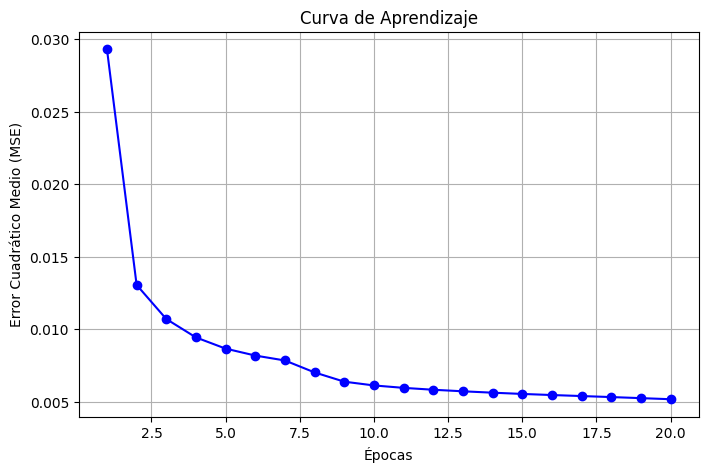
\includegraphics[width=\columnwidth]{figures/curva_ekf.png}
\caption{Curva de error del entrenamiento con EKF. El eje vertical,
rotulado como MSE, corresponde a la energía promedio del error
$E_{\text{av}}$.}
\label{fig:eav}
\end{figure}

\subsection{Comportamiento de $\mathbf{P}$ y $\mathbf{K}$}
La Fig.~\ref{fig:pk} muestra la traza de $\mathbf{P}$ y la norma de
Frobenius de $\mathbf{K}$ registradas al final de cada época. La traza
inicial es $\operatorname{tr}(\mathbf{P}(0))=46\cdot100=4\,600$ y al
terminar la primera época vale $750.1$, es decir, la incertidumbre total se
redujo $84\%$ durante la primera pasada, que es cuando el filtro extrae la
mayor parte de la información. Posteriormente la traza crece de forma
aproximadamente lineal hasta $1\,780.5$ en la época $20$, con un descenso
aislado en la época $8$, de $1\,250.1$ a $1\,166.9$.

Este crecimiento se explica por el término $\mathbf{Q}$. Cada actualización
suma $\operatorname{tr}(\mathbf{Q})=46\cdot0.001=0.046$ a la traza, lo que
equivale a $229.9$ por época, mientras que el incremento neto observado fue
de $54.2$ por época en promedio. El término de corrección
$\mathbf{K}\mathbf{H}^\top\mathbf{P}$ retira entonces alrededor de $176$ por
época, menos de lo que aporta $\mathbf{Q}$. La covarianza no alcanzó un
estado estacionario en $20$ épocas, lo cual indica que $q=0.001$ es un valor
relativamente alto para este problema. Una interpretación posible es que la
incertidumbre se acumula en las direcciones del espacio de pesos que los
datos excitan poco, por ejemplo las asociadas a neuronas saturadas, donde
$\varphi'\approx0$ y el Jacobiano aporta poca información.

La norma de la ganancia se mantuvo entre $0.060$ y $0.119$ y no decrece de
forma monótona. Debe considerarse que se registra únicamente la ganancia
del último patrón de cada época, por lo que la gráfica describe el orden de
magnitud de $\mathbf{K}$ y no su evolución patrón a patrón. A pesar de que
$\operatorname{tr}(\mathbf{P})$ aumenta, el error continuó descendiendo
durante las $20$ épocas.

\begin{figure}[htbp]
\centering
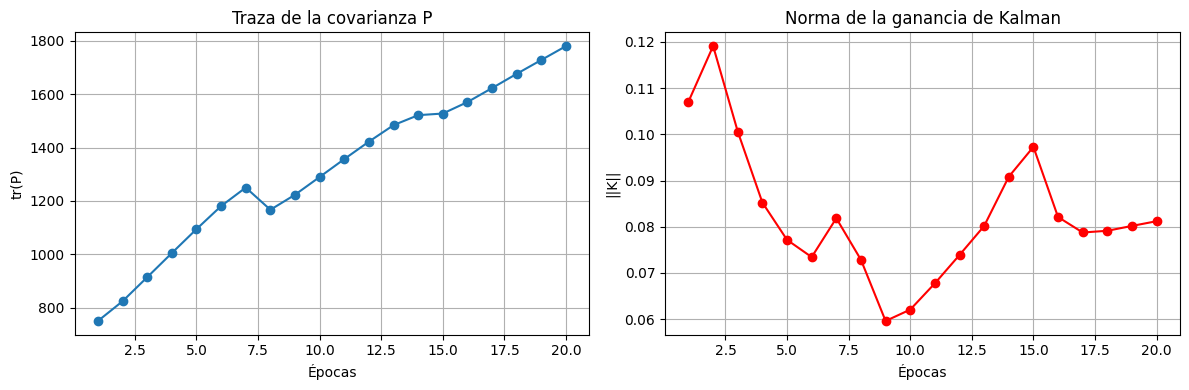
\includegraphics[width=\columnwidth]{figures/traza_p_norma_k.png}
\caption{Traza de la covarianza $\mathbf{P}$ y norma de la ganancia de
Kalman $\mathbf{K}$ al final de cada época.}
\label{fig:pk}
\end{figure}

\subsection{Desempeño en entrenamiento y prueba}
El Cuadro~\ref{tab:desempeno} presenta los resultados de ambos métodos. El
EKF alcanzó una exactitud de $99.42\%$ en entrenamiento y de $99.44\%$ en
prueba,
\begin{align*}
    \text{Accuracy}_{\text{prueba}}=\frac{1\,242}{1\,249}\times100\%=99.44\%,
\end{align*}
frente a $97.52\%$ y $97.12\%$ de retropropagación. La diferencia más
notable se encuentra en la clase $C_1$: retropropagación no reconoció ningún
patrón de bajo peso, mientras que el EKF clasificó correctamente $69$ de
$70$ en entrenamiento y $15$ de $15$ en prueba. Dado que la clase solo
cuenta con $15$ patrones de prueba, el $100\%$ debe interpretarse con
cautela, aunque el resultado de entrenamiento es consistente con él.

\begin{table}[htbp]
\caption{Resultados en entrenamiento y prueba de ambos métodos}
\label{tab:desempeno}
\begin{center}
\setlength{\tabcolsep}{4pt}
\begin{tabular}{lrrrr}
\toprule
 & \multicolumn{2}{c}{\textbf{Retropropagación}} & \multicolumn{2}{c}{\textbf{EKF}} \\
\cmidrule(lr){2-3}\cmidrule(lr){4-5}
\textbf{Métrica} & \textbf{Entren.} & \textbf{Prueba} & \textbf{Entren.} & \textbf{Prueba} \\
\midrule
Patrones          & $4\,997$  & $1\,249$  & $4\,997$  & $1\,249$ \\
Correctos         & $4\,873$  & $1\,213$  & $4\,968$  & $1\,242$ \\
Incorrectos       & $124$     & $36$      & $29$      & $7$ \\
Exactitud global  & $97.52\%$ & $97.12\%$ & $99.42\%$ & $99.44\%$ \\
\midrule
Acierto $C_1$     & $0.00\%$  & $0.00\%$  & $98.57\%$ & $100.00\%$ \\
Acierto $C_2$     & $98.64\%$ & $98.43\%$ & $98.64\%$ & $99.22\%$ \\
Acierto $C_3$     & $98.96\%$ & $97.36\%$ & $99.24\%$ & $98.90\%$ \\
Acierto $C_4$     & $98.98\%$ & $99.05\%$ & $100.00\%$ & $100.00\%$ \\
\bottomrule
\end{tabular}
\end{center}
\end{table}

La matriz de confusión del EKF en el conjunto de prueba se muestra en el
Cuadro~\ref{tab:cm} y en la Fig.~\ref{fig:cm}; entre paréntesis se incluyen
los valores de retropropagación. Los siete errores del EKF ocurren entre
clases adyacentes.

\begin{table}[htbp]
\caption{Matriz de confusión en el conjunto de prueba: EKF y, entre paréntesis, retropropagación}
\label{tab:cm}
\begin{center}
\setlength{\tabcolsep}{3pt}
\begin{tabular}{c|cccc|r}
\toprule
 & $\hat{C}_1$ & $\hat{C}_2$ & $\hat{C}_3$ & $\hat{C}_4$ & \textbf{Acierto EKF} \\
\midrule
$C_1$ & $15$ ($0$) & $0$ ($15$)    & $0$ ($0$)     & $0$ ($0$)     & $100.00\%$ \\
$C_2$ & $0$ ($0$)  & $253$ ($251$) & $2$ ($4$)     & $0$ ($0$)     & $99.22\%$ \\
$C_3$ & $0$ ($0$)  & $1$ ($4$)     & $449$ ($442$) & $4$ ($8$)     & $98.90\%$ \\
$C_4$ & $0$ ($0$)  & $0$ ($0$)     & $0$ ($5$)     & $525$ ($520$) & $100.00\%$ \\
\bottomrule
\end{tabular}
\end{center}
\end{table}

\begin{figure}[htbp]
\centering
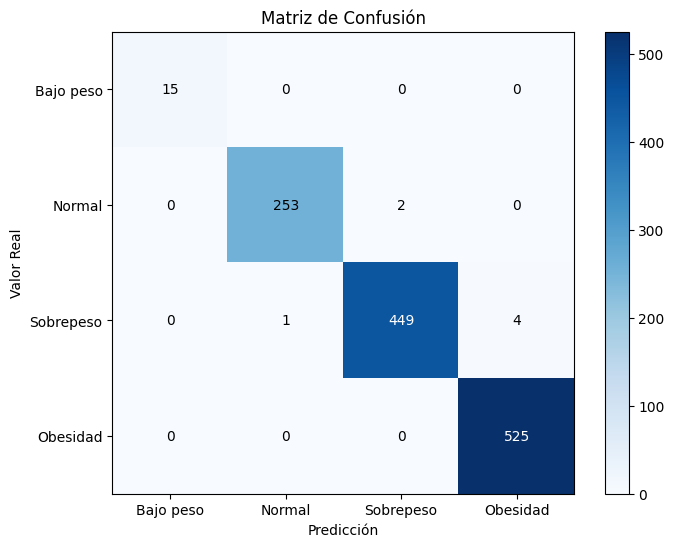
\includegraphics[width=0.85\columnwidth]{figures/matriz_confusion_ekf.png}
\caption{Matriz de confusión de la red entrenada con EKF en el conjunto de
prueba.}
\label{fig:cm}
\end{figure}

Seis de los siete errores corresponden a patrones situados a menos de $0.5$
unidades de IMC de un umbral, como se observa en el
Cuadro~\ref{tab:ejemplos}; cinco de ellos se encuentran a menos de $0.05$.
El error restante es el registro de $2.222$ m, valor de estatura que
coincide con el código de no respuesta $222.2$ cm que el filtro de rango no
eliminó y que ya había sido identificado en la Práctica~3.

\begin{table}[htbp]
\caption{Patrones de prueba mal clasificados por el EKF}
\label{tab:ejemplos}
\begin{center}
\begin{tabular}{ccccc}
\toprule
$h$ [m] & $m$ [kg] & \textbf{IMC} & \textbf{Real} & \textbf{Predicha} \\
\midrule
$1.721$ & $73.95$  & $24.968$ & $C_2$ & $C_3$ \\
$2.222$ & $118.45$ & $23.991$ & $C_2$ & $C_3$ \\
$1.556$ & $60.55$  & $25.009$ & $C_3$ & $C_2$ \\
$1.862$ & $103.10$ & $29.737$ & $C_3$ & $C_4$ \\
$1.470$ & $64.75$  & $29.964$ & $C_3$ & $C_4$ \\
$1.464$ & $64.20$  & $29.954$ & $C_3$ & $C_4$ \\
$1.463$ & $64.20$  & $29.995$ & $C_3$ & $C_4$ \\
\bottomrule
\end{tabular}
\end{center}
\end{table}

\subsection{Regiones de decisión}
Las Figs.~\ref{fig:reg_test} y \ref{fig:reg_train} muestran el mapa de
regiones de decisión del EKF en el espacio de entradas estandarizadas,
construido con una malla de separación $0.05$, junto con los patrones de
prueba y de entrenamiento. A diferencia del mapa obtenido con
retropropagación en la Práctica~3, que contenía únicamente tres regiones,
el EKF formó cuatro: aparece una región para la clase bajo peso en la parte
inferior del plano, delimitada por una tercera frontera que corresponde a
la curva teórica $m=18.5h^2$. Las tres fronteras crecen con la altura, lo
cual es coherente con las parábolas teóricas $m=18.5h^2$, $m=25h^2$ y
$m=30h^2$, y en la zona donde se concentran los datos resultan casi rectas
porque la curvatura de dichas parábolas es pequeña en ese intervalo. Las
fronteras entre peso normal, sobrepeso y obesidad se ubican en la misma zona
que las aprendidas por retropropagación.

\begin{figure}[htbp]
\centering
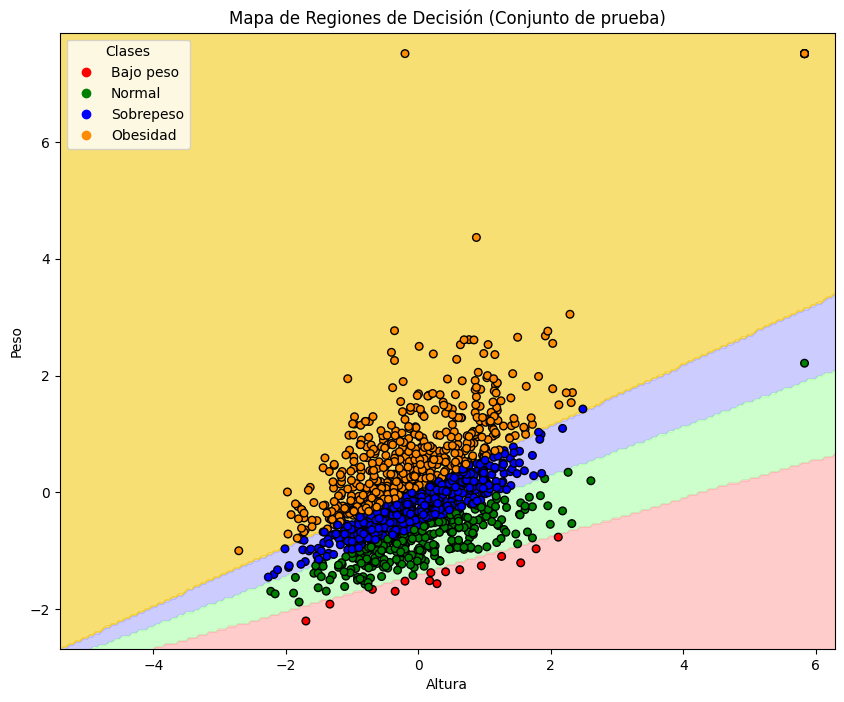
\includegraphics[width=\columnwidth]{figures/regiones_test_ekf.png}
\caption{Regiones de decisión de la red entrenada con EKF en el espacio
estandarizado, con los patrones del conjunto de prueba.}
\label{fig:reg_test}
\end{figure}

\begin{figure}[htbp]
\centering
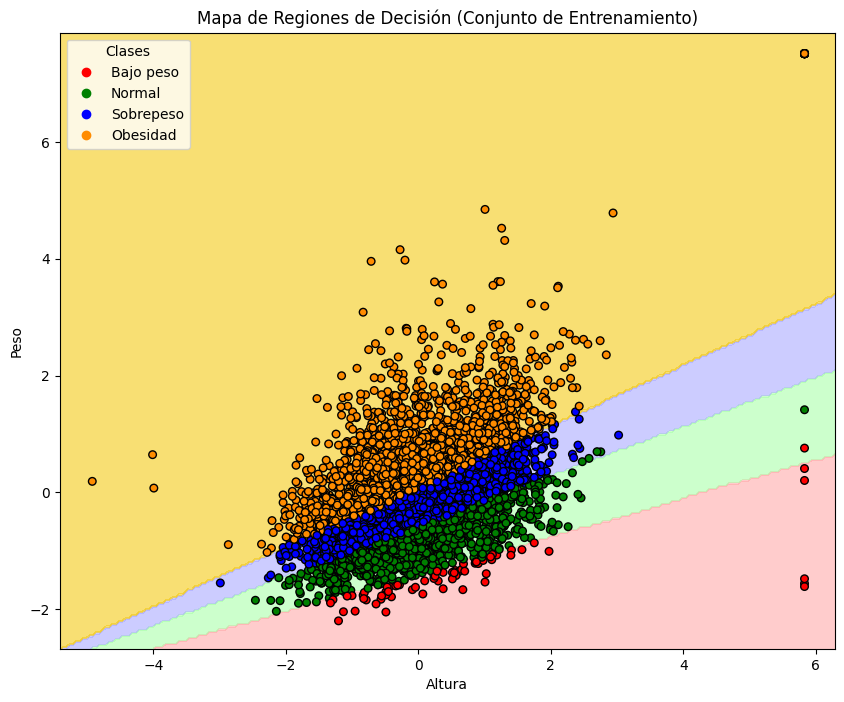
\includegraphics[width=\columnwidth]{figures/regiones_train_ekf.png}
\caption{Regiones de decisión de la red entrenada con EKF en el espacio
estandarizado, con los patrones del conjunto de entrenamiento.}
\label{fig:reg_train}
\end{figure}

\subsection{Comparación con retropropagación}
La Fig.~\ref{fig:comp} superpone las curvas de error de ambos métodos en
escala logarítmica y el Cuadro~\ref{tab:comp} resume la comparación. El
error de retropropagación desciende gradualmente: $0.3246$ en la primera
época, $0.0874$ en la época $20$ y $0.0266$ en la época $200$. El EKF
termina su primera época en $0.0293$, prácticamente el valor final de
retropropagación, y desde la segunda época, con $0.0131$, se mantiene por
debajo de él. Los tiempos se midieron en Google Colab con ambos
entrenamientos ejecutados en la misma sesión.

\begin{figure}[htbp]
\centering
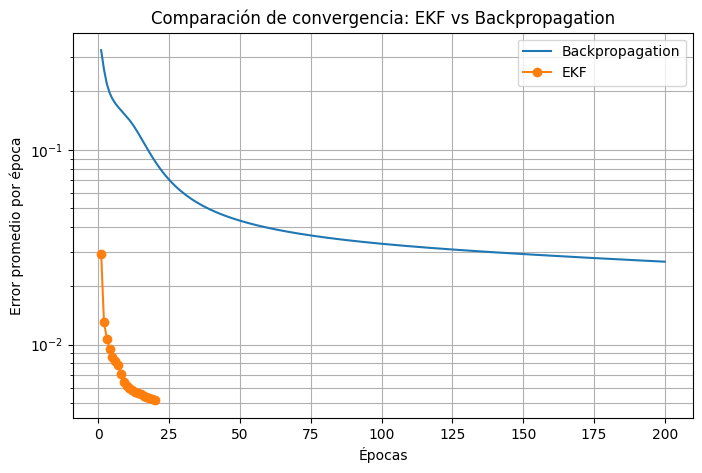
\includegraphics[width=\columnwidth]{figures/comparacion_error.png}
\caption{Curvas de error por época de retropropagación y EKF, en escala
logarítmica, con los mismos pesos iniciales.}
\label{fig:comp}
\end{figure}

\begin{table}[htbp]
\caption{Comparación entre retropropagación y EKF}
\label{tab:comp}
\begin{center}
\setlength{\tabcolsep}{4pt}
\begin{tabular}{>{\raggedright\arraybackslash}p{0.34\columnwidth}>{\raggedright\arraybackslash}p{0.26\columnwidth}>{\raggedright\arraybackslash}p{0.26\columnwidth}}
\toprule
\textbf{Criterio} & \textbf{Retropropagación} & \textbf{EKF} \\
\midrule
Arquitectura & 2--6--4 & 2--6--4 \\
Error final de entrenamiento & $0.0266$ & $0.0052$ \\
Exactitud de entrenamiento & $97.52\%$ & $99.42\%$ \\
Exactitud de prueba & $97.12\%$ & $99.44\%$ \\
Épocas hasta el criterio de paro & $200$ & $20$ \\
Tiempo total de entrenamiento & $53.28$ s & $30.22$ s \\
Tiempo por época & $0.266$ s & $1.511$ s \\
Errores de prueba por clase & $15$, $4$, $12$, $5$ & $0$, $2$, $5$, $0$ \\
Sensibilidad a parámetros de diseño & Un parámetro, $\eta$ & Cuatro: $p_0$, $q$, $r$, $\eta$; estable en el intervalo probado \\
Memoria por actualización & $L=46$ valores & $\mathbf{P}$: $L^2=2\,116$ valores \\
Complejidad de implementación & Baja: gradientes locales y regla delta & Mayor: vector de pesos, Jacobiano y álgebra matricial \\
\bottomrule
\end{tabular}
\end{center}
\end{table}

\subsection{Sensibilidad a los parámetros de diseño}
\label{sec:sens}
Para evaluar la sensibilidad del EKF se repitió el entrenamiento durante
$10$ épocas, con los mismos pesos iniciales, modificando un parámetro a la
vez respecto a la configuración base. El Cuadro~\ref{tab:sens} muestra los
resultados.

\begin{table}[htbp]
\caption{Sensibilidad del EKF a sus parámetros de diseño, 10 épocas}
\label{tab:sens}
\begin{center}
\setlength{\tabcolsep}{3.5pt}
\begin{tabular}{rrrrcccc}
\toprule
$p_0$ & $q$ & $r$ & $\eta$ & $E_{\text{av}}(1)$ & $E_{\text{av}}(10)$ & \textbf{Prueba} & $C_1$ \\
\midrule
$100$    & $10^{-3}$ & $1$   & $1$   & $0.0293$ & $0.0061$ & $99.52\%$ & $15/15$ \\
\midrule
$1$      & $10^{-3}$ & $1$   & $1$   & $0.0711$ & $0.0121$ & $98.40\%$ & $0/15$ \\
$10^{4}$ & $10^{-3}$ & $1$   & $1$   & $0.0421$ & $0.0051$ & $99.52\%$ & $15/15$ \\
\midrule
$100$    & $0$       & $1$   & $1$   & $0.0323$ & $0.0083$ & $98.96\%$ & $14/15$ \\
$100$    & $10^{-5}$ & $1$   & $1$   & $0.0323$ & $0.0075$ & $99.60\%$ & $15/15$ \\
$100$    & $10^{-1}$ & $1$   & $1$   & $0.0300$ & $0.0121$ & $98.56\%$ & $15/15$ \\
\midrule
$100$    & $10^{-3}$ & $0.1$ & $1$   & $0.0316$ & $0.0078$ & $99.36\%$ & $15/15$ \\
$100$    & $10^{-3}$ & $10$  & $1$   & $0.0442$ & $0.0106$ & $98.72\%$ & $15/15$ \\
\midrule
$100$    & $10^{-3}$ & $1$   & $0.5$ & $0.0384$ & $0.0069$ & $99.52\%$ & $15/15$ \\
$100$    & $10^{-3}$ & $1$   & $0.1$ & $0.1243$ & $0.0177$ & $98.40\%$ & $11/15$ \\
\bottomrule
\end{tabular}
\end{center}
\end{table}

Ninguna de las diez configuraciones divergió y todas superaron en $10$
épocas la exactitud de prueba que retropropagación obtuvo en $200$. Se
observa lo siguiente:
\begin{itemize}
    \item $p_0$: un valor pequeño, $p_0=1$, expresa poca incertidumbre
    inicial, produce correcciones débiles y fue la única configuración que
    no reconoció la clase $C_1$. Un valor muy grande, $p_0=10^4$, empeora la
    primera época, pero conduce al menor error final.
    \item $q$: con $q=0$ el filtro pierde capacidad de adaptación y el error
    final es mayor que con la configuración base; con $q=10^{-1}$ la traza de
    $\mathbf{P}$ crece hasta $6\times10^4$ y el error se duplica. Los valores
    intermedios son los más adecuados.
    \item $r$: al aumentar a $r=10$ se reduce la confianza en la innovación
    instantánea, la ganancia disminuye y la convergencia es más lenta.
    \item $\eta$: reducirla atenúa la corrección; con $\eta=0.1$ el error de
    la primera época se cuadruplica y la clase $C_1$ se reconoce solo
    parcialmente.
\end{itemize}

\section{Reflexión comparativa}

\textbf{Error bajo en menos épocas.} El EKF. Al concluir su primera época
registró $E_{\text{av}}=0.0293$, valor que retropropagación alcanzó hasta
el final de sus $200$ épocas, $0.0266$; en la época $20$ el EKF llegó a
$0.0052$, cinco veces menos que el error final de retropropagación. Esto
coincide con lo reportado en las referencias, según las cuales el
entrenamiento basado en EKF requiere menos épocas y converge más rápido que
los métodos basados en retropropagación \cite{b2,b3,b7}.

\textbf{Tiempo real de ejecución.} En este experimento el EKF también fue
más rápido en tiempo total, $30.22$ s contra $53.28$ s, pero por una razón
distinta al costo por época. Cada época del EKF tardó $1.511$ s y cada
época de retropropagación $0.266$ s, es decir, el EKF es $5.7$ veces más
costoso por época, pues para cada patrón construye un Jacobiano de
$46\times4$ y opera con una covarianza de $46\times46$. El número de épocas
no determina el tiempo total porque el costo de una época es diferente en
cada método: el tiempo es el producto de ambas cantidades. El EKF resultó
más rápido únicamente porque necesitó diez veces menos épocas, lo cual
compensó su mayor costo unitario. Si se compara el tiempo necesario para
igualar el error final de retropropagación, el EKF lo consigue en dos
épocas, aproximadamente $3$ s.

\textbf{Sensibilidad a los parámetros de ajuste.} Retropropagación tiene un
solo parámetro, $\eta$, del cual dependen por completo la velocidad y la
estabilidad; en la Práctica~3 se evaluó únicamente $\eta=0.01$. El EKF
tiene cuatro, $\eta$, $\mathbf{P}(0)$, $\mathbf{Q}$ y $\mathbf{R}$, lo que
amplía el espacio de búsqueda. Sin embargo, el Cuadro~\ref{tab:sens}
muestra que el EKF fue robusto: al variar $p_0$ en cuatro órdenes de
magnitud, $q$ desde $0$ hasta $10^{-1}$ y $r$ en dos órdenes de magnitud,
el entrenamiento convergió siempre y
la exactitud de prueba se mantuvo entre $98.40\%$ y $99.60\%$. La razón es
que la ganancia de Kalman escala la corrección de forma automática según la
incertidumbre, de modo que $\eta$ deja de ser crítica y puede fijarse en
$1$. Los parámetros con mayor efecto fueron $p_0$ pequeño y $\eta$ pequeña,
que debilitan la corrección.

\textbf{Sencillez de implementación y depuración.} Retropropagación fue más
sencilla, ya que solo requiere los gradientes locales y la regla delta, con
operaciones entre vectores. El EKF añade tres componentes. El primero es el
manejo de un vector único de parámetros, con el riesgo de que el orden de
empaquetado no coincida con el del Jacobiano. El segundo, y el más
laborioso, es la construcción de $\mathbf{H}$, que exige calcular la
sensibilidad de cada salida por separado. El tercero es el álgebra
matricial, en la que las dimensiones deben ser consistentes. Las partes que
generaron mayor dificultad fueron dos. Una fue la forma de los arreglos:
sumar un vector de forma $(46,)$ con uno de $(46,1)$ produce en NumPy una
matriz de $46\times46$ sin emitir error. La otra fue un error en la
actualización de la covarianza durante el desarrollo, por el cual
$\mathbf{P}$ permanecía constante. En ese caso la red seguía aprendiendo,
porque con $\mathbf{P}=p_0\mathbf{I}$ la corrección
$\mathbf{K}\mathbf{e}$ es proporcional a $\mathbf{H}\mathbf{e}$, que es la
dirección del descenso de gradiente, pero lo hacía con la lentitud propia
de retropropagación. Este tipo de errores no detiene la ejecución, por lo
que la depuración requirió verificar formas, comparar el Jacobiano contra
diferencias finitas y vigilar $\operatorname{tr}(\mathbf{P})$.

\textbf{Costo de almacenar y actualizar $\mathbf{P}$.} Retropropagación
almacena un gradiente por parámetro, $L=46$ valores, y su costo por patrón
es proporcional a $L$. El EKF almacena $\mathbf{P}$, con $L^2=2\,116$
valores, y cada actualización requiere los productos
$\mathbf{P}\mathbf{H}$ y $\mathbf{K}\mathbf{H}^\top\mathbf{P}$, cuyo costo
es del orden de $L^2m$, además de $m$ recorridos hacia atrás para formar
$\mathbf{H}$ y la inversión de una matriz de $m\times m$. Para esta red el
costo adicional es manejable y se refleja en el factor $5.7$ de tiempo por
época.

\textbf{Regiones de decisión.} Ambos métodos ubicaron las fronteras entre
peso normal, sobrepeso y obesidad en la misma zona del plano, cerca de las
curvas teóricas $m=25h^2$ y $m=30h^2$, y en ambos los errores se concentran
junto a dichas fronteras. La diferencia principal es la región de bajo
peso: retropropagación no la formó y asignó esos patrones a peso normal,
mientras que el EKF construyó una cuarta región en la parte inferior del
plano. Además, las fronteras del EKF son más precisas: los errores entre
$C_2$, $C_3$ y $C_4$ en prueba disminuyeron de $21$ a $7$.

\textbf{Generalización.} El EKF generalizó mejor, con $99.44\%$ en prueba
frente a $97.12\%$. La diferencia de $2.32$ puntos porcentuales equivale a
pasar de $36$ a $7$ errores en $1\,249$ patrones y es relevante por su
origen: $15$ de los $29$ errores eliminados corresponden a la clase bajo
peso, que retropropagación no detectaba, de manera que el EKF corrige una
deficiencia cualitativa del modelo y no solo mejora un promedio. En ambos
métodos la exactitud de entrenamiento y la de prueba son casi iguales, por
lo que ninguno presenta sobreajuste. Una explicación posible de la mejora
en $C_1$ es que la ganancia de Kalman pondera cada corrección con la
incertidumbre acumulada en $\mathbf{P}$, lo que permite correcciones
grandes ante los pocos patrones de esa clase, mientras que el descenso de
gradiente con $\eta$ pequeña los diluye entre miles de patrones de las
otras clases. Esta hipótesis es consistente con el
Cuadro~\ref{tab:sens}, donde las configuraciones que debilitan la
corrección, $p_0=1$ y $\eta=0.1$, son las que pierden la clase $C_1$.

\textbf{Redes con muchos más pesos.} Sería más conveniente
retropropagación. La memoria del EKF crece con $L^2$ y su costo por patrón
con $L^2m$: una red con $10^4$ pesos requeriría una covarianza de $10^8$
elementos, cerca de $800$ MB en doble precisión, y una con $10^6$ pesos
sería inviable. Retropropagación crece linealmente con $L$. Para redes
grandes el EKF solo es práctico en variantes desacopladas, que dividen
$\mathbf{P}$ en bloques por neurona o por capa a costa de ignorar parte de
las correlaciones \cite{b5}.

\textbf{Cuándo preferir cada método.} A partir de estos resultados, el EKF
es preferible cuando la red es pequeña, cuando se requiere convergencia en
pocas pasadas sobre los datos, cuando el aprendizaje debe realizarse en
línea, patrón por patrón, como en identificación y control, o cuando
existen clases o regiones del espacio poco representadas. Retropropagación
es preferible cuando la red tiene muchos parámetros, cuando la memoria es
limitada o cuando se busca una implementación simple y de bajo costo por
iteración, aunque requiera más épocas.

\textbf{Limitaciones.}
\begin{itemize}
    \item Los patrones se presentaron en el mismo orden en todas las épocas
    en ambos métodos.
    \item El criterio de paro fue un número fijo de épocas; no se
    implementó un paro basado en el error.
    \item Los tiempos corresponden a una sola ejecución en Google Colab y
    pueden variar entre ejecuciones.
    \item Con $q=0.001$ la covarianza no alcanzó un estado estacionario.
    \item La prueba de sensibilidad modificó un parámetro a la vez, con
    $10$ épocas y una sola semilla, por lo que no explora las interacciones
    entre parámetros.
    \item La clase $C_1$ cuenta solo con $15$ patrones de prueba.
\end{itemize}

\section{Conclusiones}
Se implementó desde cero el entrenamiento de un perceptrón multicapa
2--6--4 mediante el filtro extendido de Kalman, para lo cual se agruparon
los $46$ parámetros en un vector, se construyó la matriz Jacobiana de las
salidas con la regla de la cadena y se programaron las ecuaciones de
ganancia, corrección de pesos y actualización de la covarianza. Con la
misma red, los mismos datos y los mismos pesos iniciales que en la
Práctica~3, el EKF alcanzó una exactitud de prueba de $99.44\%$ en $20$
épocas, frente a $97.12\%$ de retropropagación en $200$ épocas, y un error
final cinco veces menor.

Las ventajas observadas del EKF fueron la convergencia en muchas menos
épocas, un menor tiempo total de entrenamiento en este problema, una mejor
generalización, el reconocimiento de la clase minoritaria de bajo peso y
una baja sensibilidad a la razón de aprendizaje. Sus desventajas fueron un
costo por época $5.7$ veces mayor, una memoria que crece con el cuadrado
del número de pesos, tres parámetros de diseño adicionales y una
implementación más compleja y difícil de depurar. Retropropagación ofrece
lo contrario: es simple, económica por iteración y escalable, pero converge
lentamente y, bajo las mismas condiciones, no logró aprender la clase menos
representada.

Ambos algoritmos entrenan la misma red desde interpretaciones distintas.
Retropropagación calcula el gradiente de una función de costo y desciende
por él; el EKF trata los pesos como estados desconocidos y combina la
sensibilidad de las salidas, $\mathbf{H}$, con una estimación de la
incertidumbre, $\mathbf{P}$, para calcular una corrección adaptativa. Como
trabajo futuro se propone aleatorizar el orden de los patrones, ajustar
$q$ para que la covarianza alcance un estado estacionario, añadir un
criterio de paro basado en un conjunto de validación y evaluar una versión
desacoplada del filtro en redes de mayor tamaño.

\begin{thebibliography}{00}

\bibitem{b1} \textit{Extended Kalman Filter based training algorithm}, apuntes de clase del curso Sistemas Inteligentes 3 -- Redes Neuronales Artificiales, CUCEI, Universidad de Guadalajara, 2026.

\bibitem{b2} J. D. Rios, A. Y. Alanis, C. Lopez-Franco, and N. Arana-Daniel, ``RHONN identifier-control scheme for nonlinear discrete-time systems with unknown time-delays,'' \textit{Journal of the Franklin Institute}, vol. 355, pp. 218--249, 2018, doi: 10.1016/j.jfranklin.2017.11.014.

\bibitem{b3} J. Hernandez-Barragan, J. D. Rios, A. Y. Alanis, C. Lopez-Franco, J. Gomez-Avila, and N. Arana-Daniel, ``Adaptive single neuron anti-windup PID controller based on the extended Kalman filter algorithm,'' \textit{Electronics}, vol. 9, no. 4, art. 636, 2020, doi: 10.3390/electronics9040636.

\bibitem{b4} J. O. Estrada, J. D. Rios, and A. Y. Alanis, ``Adaptive neural PID outer-loop control for quadcopter UAVs with asymmetric saturation,'' \textit{Eng}, vol. 7, art. 460, 2026, doi: 10.3390/eng7090460.

\bibitem{b5} S. Haykin, \textit{Neural Networks and Learning Machines}, 3rd ed. Upper Saddle River, NJ, USA: Pearson/Prentice Hall, 2009.

\bibitem{b6} Instituto Nacional de Salud Pública, ``Encuesta Nacional de Salud y Nutrición Continua 2022 (ENSANUT 2022): base de datos de antropometría,'' Cuernavaca, México: INSP, 2023. [En línea]. Disponible: https://ensanut.insp.mx

\bibitem{b7} S. Singhal and L. Wu, ``Training multilayer perceptrons with the extended Kalman algorithm,'' in \textit{Advances in Neural Information Processing Systems 1}, 1988.

\end{thebibliography}

\end{document}
